% Editable LaTeX manuscript. Compile: latexmk -pdf atfm-paper.tex
\documentclass[11pt,a4paper]{article}
\usepackage[margin=24mm]{geometry}
\usepackage[T1]{fontenc}
\usepackage[utf8]{inputenc}
\usepackage{newtxtext,newtxmath}
\usepackage{microtype}
\usepackage{graphicx}
\usepackage{booktabs,tabularx,array,makecell}
\usepackage{caption}
\usepackage{amsmath}
\usepackage{needspace}
\usepackage{fvextra}
\usepackage[section]{placeins}
\usepackage[numbers,sort&compress]{natbib}
\usepackage{xurl}
\usepackage[hidelinks]{hyperref}
\hypersetup{pdftitle={Agent Traffic Flow Management: Forecasting and Admission Control for LLM Agent Fleets},pdfauthor={Alexander Aghili}}
\graphicspath{{latex-fig/}}
\captionsetup{font=small,labelfont=bf,skip=6pt}
\renewcommand{\theadfont}{\small\bfseries}
\renewcommand{\arraystretch}{1.13}
\setlength{\parindent}{1em}
\setlength{\parskip}{3pt}
\setlength{\emergencystretch}{1em}
\setcounter{topnumber}{3}
\setcounter{bottomnumber}{2}
\setcounter{totalnumber}{5}
\renewcommand{\topfraction}{.9}
\renewcommand{\bottomfraction}{.8}
\renewcommand{\textfraction}{.08}
\renewcommand{\floatpagefraction}{.75}
\title{\textbf{Agent Traffic Flow Management}\\[5pt]\large Forecasting and Admission Control for LLM Agent Fleets}
\author{Alexander Aghili}
\date{Research report\enspace\textperiodcentered\enspace September 27, 2026}
\begin{document}
\maketitle

\begin{abstract}
Large language model (LLM) agents alternate between inference and external tool execution. A serving system can therefore observe sessions that are likely to generate future requests before those requests arrive. We investigate whether this information improves aggregate demand forecasts and whether acting on the forecasts benefits latency-sensitive sessions. Agent Traffic Flow Management (ATFM) combines a session-state demand model, a tool-progress sidecar, and an admission proxy that can defer background requests. Across two public coding-agent corpora, the ratio of Kalman-baseline loss to elapsed-time-model loss ranges from 1.96 to 5.43 at five-minute horizons and from 2.73 to 5.09 at fifteen-minute horizons, using the 0.9-quantile pinball loss averaged over three seeds. In a separate collection of long-running tools, progress information reduces mean pinball loss from 24.9 to 8.9 seconds. Closed-loop simulation exposes a conditional benefit: in a loaded regime with short interactive tools, forecast-based holds improve session-weighted service-level-objective attainment by 9.3 percentage points while increasing mean background completion time by approximately 24\%. A regime with long interactive tools and a shorter hold cap does not establish an advantage over rules-based admission, and a controlled cap ablation in the loaded regime removes the gain entirely: at a 60-second cap the forecast arms' SLO differences from native span zero while their background costs remain, and a same-rule lookahead fed true demand does no better. These findings support session-aware forecasting but show that the measured policy gain came from long deferral of background work rather than from forecast accuracy, and that this hold heuristic collapses to holding everything under load. Serving results remain conditional on an unvalidated simulator and require hardware evaluation.


\end{abstract}
\textbf{Keywords:} LLM serving; agent workloads; probabilistic forecasting; admission control; KV cache.


\section{Introduction}
\label{sec:1}
An LLM agent typically executes a sequence of model calls and external actions: a generated response invokes a tool, the tool produces a result, and that result becomes part of a subsequent prompt. While the tool runs, the session does not require inference compute, but its retained key-value (KV) cache may reduce the cost of resumption. Concurrent agents consequently create a scheduling problem that spans both requests already queued at the engine and sessions executing outside it.


Our premise is that the latter group provides useful information about future demand. A session's current phase, elapsed tool time, context length, and available progress reports constrain when it may next request inference. This information is particularly relevant when many active sessions share a serving pool. It is less useful when new sessions dominate arrivals, external actions are unobservable, or uncertainty in return times overwhelms the controller's decision horizon.


ATFM maintains a \emph{demand board} that aggregates per-session return-time distributions into forecasts of prompt-token and KV-block demand. An admission proxy uses these forecasts to delay deferrable work when interactive demand is expected to exceed available capacity. The name refers to the separation between demand prediction and ground-delay decisions in air-traffic flow management; the implemented controller is a heuristic, without an optimality or service-level guarantee.


This report makes three contributions. First, it defines and implements a common forecast interface that separates the value of request history, elapsed tool time, and live progress. Second, it evaluates these information sources using held-out coding-agent traces and instrumented tool executions. Third, it measures the latency and background-completion trade-off of forecast-based holds in closed-loop simulation, including a no-hold ablation and a regime in which the policy does not outperform a simpler alternative. Forecast evaluation and policy evaluation are kept distinct because changing admission times changes subsequent agent arrivals.


The evidence addresses three research questions: \textbf{H1a}, whether in-flight session state improves fleet-demand forecasting over aggregate history; \textbf{H1b}, whether progress improves remaining-time prediction beyond elapsed time; and \textbf{H2}, whether forecast-based admission improves interactive latency at an explicitly measured cost to background work. The implementation and experiment records are described in Appendix~\ref{app:A}.


\section{Background and Related Work}
\label{sec:2}
\textbf{Program-aware serving.} ThunderAgent represents multi-turn workflows as programs and coordinates inference and tool resources \citep{r1}. Continuum retains selected KV caches under a time-to-live policy that accounts for reload cost and queueing delay \citep{r2}. These systems establish that an agent's state beyond its current request can inform serving decisions. ATFM instead evaluates aggregate demand over explicit horizons and uses that forecast to control admission. Its per-tool history predictor and working-set policy are local baselines, not reproductions of Continuum or ThunderAgent; their results cannot be read as comparisons against the full published systems.


\textbf{Tool signals and reactive scheduling.} Liu et al. recover live tool progress for cache-management decisions \citep{r3}, directly motivating the information source studied in H1b. ATFM does not claim novelty for extracting progress. Its focus is the aggregation of session-level predictions and the conditions under which those predictions help a fleet controller. Conversely, ConServe emphasizes conversation-level observation and disaggregated scheduling rather than duration prediction \citep{r4}. This alternative motivates the rules-only baseline and the explicit separation of prediction quality from policy effectiveness.


\textbf{Infrastructure and workload evidence.} NVIDIA Dynamo provides agent-oriented serving mechanisms, including request hints, scheduling, and KV-aware infrastructure \citep{r5}. ATFM's prototype integrates a proxy with Dynamo's Mocker path; the simulation experiments use a separate local engine model. DSec demonstrates large-scale, stateful sandbox execution decoupled from GPU training \citep{r6}. Its reported scale, approximately three million sandboxes per day and more than 380,000 concurrent sandboxes, motivates studying external execution state, but does not establish that inference demand is forecastable. TraceLab \citep{r7} and the SemiAnalysis AgentX corpus \citep{r8} supply the real session traces used here.


\section{Demand Model and Forecasting Method}
\label{sec:3}
\subsection{Forecast target}
\label{sec:3.1}
At time \(t\), let \(A_{c}(t)\) denote known sessions in class \(c\), where the classes are interactive and background. For session \(i\), let \(R_{i}(t)\) be the time until its next model request and \(L_{i}\) the input-token count of that request. With block size \(b\) = 16 tokens, the KV-demand forecast is


\begin{equation}
D^{\mathrm{KV}}_c(t,h) = \sum_{i\in A_c(t)} \mathbf{1}\!\left[R_i(t)\leq h\right]\left\lceil\frac{L_i}{b}\right\rceil + U^{\mathrm{KV}}_c(t,h).
\label{eq:1}
\end{equation}
The term \(U\) represents demand from future sessions, including modeled child sessions and exogenous arrivals. Replacing \(\lceil L_i/b\rceil\) with \(L_{i}\) gives the prompt-token target. Each session contributes only its first request in a horizon. Thus, these targets measure first-resumption demand, not all requests in the interval, instantaneous resident KV occupancy, or cache-miss-adjusted prefill work. The distinction matters because retention, prefix sharing, and repeated calls can change actual memory and compute requirements.


Known context length informs the next prompt size, but the size increment from tool output must be predicted. The live proxy also uses a character-count approximation when token counts are unavailable. Context size is therefore not assumed to be known exactly in deployment.


\subsection{State and predictor hierarchy}
\label{sec:3.2}
The registry distinguishes model execution, tool execution, and a pending phase between tool completion and the next request. Events carry session identity, workload class, timestamps, tool identity, backend identity, and optional progress or data signals. Trace adapters map these events to a common table with one row per model call and its associated tool phase. Pending gaps are modeled separately; treating every completed tool as an immediate request would systematically misrepresent human and harness delays.


\begin{table}[!htbp]
\centering
\caption{Forecast models and the information available to each. All session models use the same aggregation procedure.}
\label{tab:1}
\small
\setlength{\tabcolsep}{4pt}
\begin{tabularx}{\linewidth}{@{}p{.22\linewidth}X@{}}
\toprule
\thead[l]{Model} & \thead{Information and prediction rule} \\
\midrule
B0: persistence & Point forecast equal to the most recently realized demand window. \\
B1: Kalman & Local linear trend over realized demand; predictive Gaussian samples clipped at zero. \\
B2: history & Unconditional empirical tool-duration samples, minus elapsed time and clipped at zero. \\
M1: survival & Tool-duration samples conditioned on the tool still running at the current elapsed time. \\
M2: progress & M1 augmented with progress-rate estimation and a learned mapping from reported progress to elapsed-time fraction. \\
M3: backend & Progress prediction augmented with a shared backend slowdown factor; exploratory only. \\
\bottomrule
\end{tabularx}
\end{table}


B2 uses elapsed time in the final subtraction but does not condition its duration distribution on survival. For tool duration \(T\) and elapsed time \(e\), the idealized survival model instead uses


\begin{equation}
\Pr(T-e>r\mid T>e)=\frac{S(e+r)}{S(e)},\qquad r\geq0,
\label{eq:2}
\end{equation}
where \(S\) is the survival function. The implementation uses empirical duration distributions with finite-sample fallbacks, adds a tool-to-request gap, and assigns probability mass to sessions that do not return. M2 combines a rate filter with empirical progress curves because a tool's reported fraction complete need not be linear in wall-clock time. When progress is absent, M2 falls back to the elapsed-time model.


\subsection{Aggregation and calibration}
\label{sec:3.3}
The demand board draws Monte Carlo return times and next-call sizes, then sums their contributions using Equation~\eqref{eq:1}. It models one level of child-session fan-out and a Poisson process for exogenous arrivals. The arrival rate is estimated from recent session starts; first-call sizes are sampled from training data. History-only predictors receive a realized demand window only after its full horizon has elapsed, preventing future-window leakage.


Forecast dispersion can be calibrated by fitting a variance-inflation factor separately for each class and horizon on a held-out portion of the training data. Calibration uses an overlaid fleet at the evaluation arrival rate. This adjustment changes interval width, but it does not guarantee calibration under model bias, dependence between sessions, or workload shift. M3 is implemented but is not a basis for the main claims: an earlier synthetic slowdown experiment showed inconsistent gains across horizons.


\section{System and Admission Policy}
\label{sec:4}
\subsection{Architecture and prototype}
\label{sec:4.1}
Figure~\ref{fig:1} separates the request path from the measurement and control path. The sidecar observes tool output and emits structured events while preserving the subprocess result. The demand board consumes events and publishes forecast samples. The proxy maintains an admission window and applies ordering and hold decisions before forwarding requests to the serving engine. The Python prototype includes in-memory and JSONL event buses, a FastAPI proxy, a live board, corpus adapters, and a discrete-event simulator. Redis-based deployment, explicit KV placement, and replica-floor control remain architectural extensions.


\begin{figure}[!htbp]
\centering
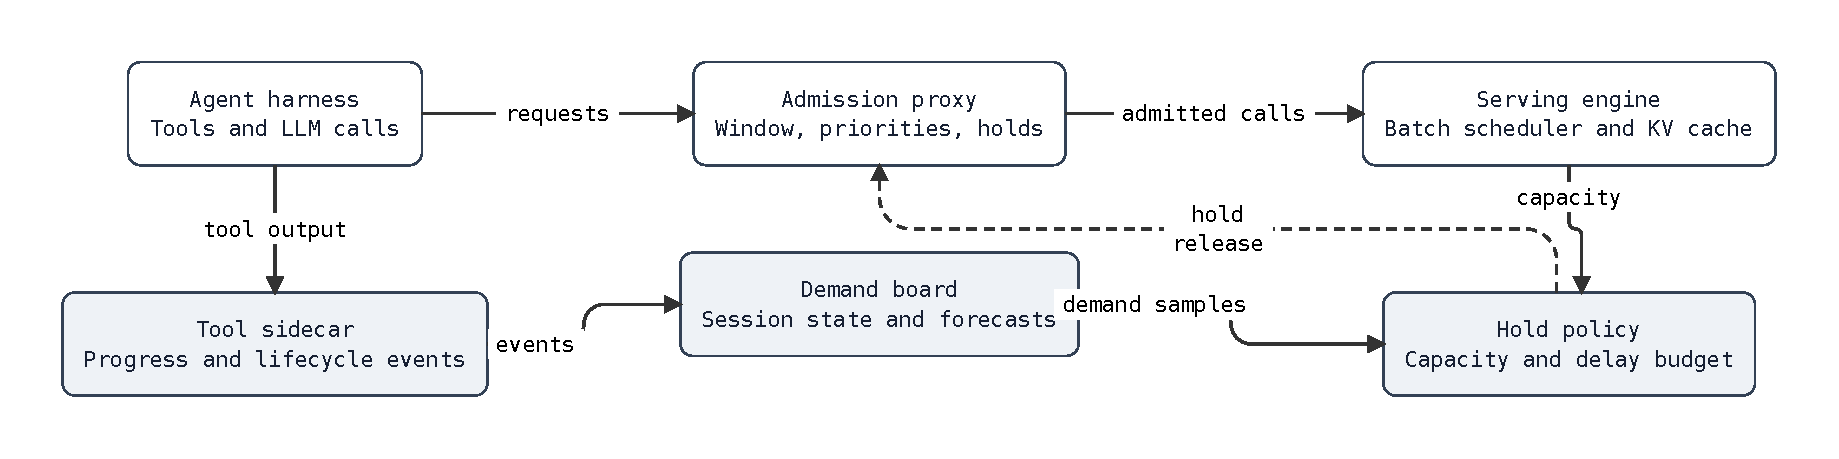
\includegraphics[width=1\linewidth]{system.pdf}
\caption{ATFM's logical architecture. The upper row carries model requests; the lower row carries tool state, forecasts, and capacity information. The dashed connection denotes control of admission. The simulator exercises the feedback loop; the Dynamo Mocker experiment verifies request integration rather than real-GPU capacity feedback.}
\label{fig:1}
\end{figure}


The sidecar parses build percentages, test counters, generic work counters, and output-rate signals. Parser and event-publication failures are handled without changing tool output. The proxy accepts external hold directives and falls back to default predictions if the prediction service fails; this does not imply that an unavailable serving backend can be bypassed. The recorded Mocker test exercised three concurrent scripted sessions, a two-request admission window, and deadline-sensitive priority hints. It did not measure GPU memory behavior, model quality, or end-to-end controller effectiveness on hardware.


\subsection{Ordering and admission}
\label{sec:4.2}
A global window bounds requests released to the engine. Waiting calls are ordered first by class and deadline tier, then by an index. Interactive calls receive tier 1, or tier 2 when estimated deadline slack is below a threshold; background calls receive tier 0. Within a tier, the index is


\begin{equation}
\pi_i=\frac{w_{c(i)}\left(1+\beta\,\mathbb{E}[T_{\mathrm{next},i}]\right)}{\mathbb{E}[S_i]},
\label{eq:3}
\end{equation}
where \(w_{c(i)}\) is the class weight, \(S_{i}\) is model service time, and \(T_{next,i}\) is the next tool duration. The coefficient \emph{\(\beta\)} controls the preference for serving sessions that will subsequently spend time outside the engine. Service time is estimated from prompt and output lengths using configured prefill and decode rates. Rules-only admission sets the next-tool term to zero. This index is a heuristic, not a Gittins-index solution or an optimal scheduling policy.


\subsection{Forecast-based holds and their costs}
\label{sec:4.3}
The GDP-lite policy consults a 30-second forecast slot when a background call becomes eligible for admission. It holds the call if either the 0.9 quantile of interactive KV demand exceeds capacity not occupied by running requests, or an approximation to average interactive batch occupancy exceeds free batch slots. The occupancy approximation divides forecast prompt tokens by mean prompt size to estimate call count, then multiplies by expected service time and divides by slot duration. These tests approximate resource pressure; neither directly enforces a probabilistic bound on actual simultaneous occupancy.


Holds are reconsidered at expiry and capped relative to request arrival. Expiration of the policy hold does not bypass the admission window, so ordinary queueing can continue after the cap. The simulator separately records policy-hold duration, ordinary queueing, held-cache occupancy integrated over time, displacement evictions, and prefix recomputation. A delay limit consequently bounds imposed hold time, not total request latency or session completion time.


The completed loaded experiment uses a 600-second hold cap. The long-interactive-tool experiment uses 60 seconds. Where the admission window equals engine batch capacity, the window-based arms place their backlog at the proxy. The native arm queues at the engine. This queue placement is part of the treatment, and results do not isolate the effect of engine-side priority hints.


\section{Experimental Methodology}
\label{sec:5}
\subsection{Data and splits}
\label{sec:5.1}
\begin{table}[!htbp]
\centering
\caption{Data sources and evaluation units. Corpus counts describe the repository's recorded input snapshot rather than a guarantee about current upstream releases.}
\label{tab:2}
\small
\setlength{\tabcolsep}{4pt}
\begin{tabularx}{\linewidth}{@{}p{.17\linewidth}p{.28\linewidth}X@{}}
\toprule
\thead{Source} & \thead{Recorded size} & \thead{Evaluation protocol} \\
\midrule
TraceLab \citep{r7} & 4,265 sessions; approximately 357,000 model steps & H1a: 30\% of calendar-week blocks held out; test sessions overlaid as a Poisson fleet. \\
AgentX \citep{r8} & 393 root sessions; 1,697 sub-agent groups & H1a: 30\% of session families held out; roots and children split and shifted together. \\
Instrumented tools & 202 observation points per model across nine scored job families & H1b: one job family held out at a time; real builds, pipelines, and NumPy tests. \\
Synthetic programs & Four completed regimes; three seeds per regime & H2: one hour of new-session arrivals, followed by completion; matched programs across policy arms. \\
\bottomrule
\end{tabularx}
\end{table}


H1a uses arrival rates of 100, 200, and 400 sessions per hour, four-hour overlay windows, 30-second forecast ticks, 256 Monte Carlo samples, and horizons of 10, 30, 120, 300, and 900 seconds. The seed controls splitting and overlay generation. Both public corpora are assigned to the interactive class by their adapters, so these measurements are not evidence for forecast accuracy across independently labeled interactive and background populations.


TraceLab's adapter aggregates tools launched by a model step into one phase and uses the longest tool to label that phase. AgentX's inter-request gaps are not individually labeled as tool or human time; they are represented as generic gaps unless associated with a sub-agent group. Keeping families together prevents related root and child traces from crossing the train/test boundary, but Poisson overlays do not preserve production arrival correlations.


H1b scores observations every 15 seconds within tool phases longer than 30 seconds. A job family is defined by the collection job name, so the same tool at other sizes or rates may remain in training. The retained score file contains nine families: two fmt build variants, four linear pipelines, two staged pipelines, and the NumPy suite. All observations in a held-out family are scored using models trained on the remaining families. Results are averaged over observation points; long phases therefore receive more weight, and the 202 points are not independent experimental replicates.


\Needspace{10\baselineskip}
\subsection{Forecast metrics}
\label{sec:5.2}
The primary forecast metric is pinball loss at quantile \emph{\(\tau\)} = 0.9, with supplementary continuous ranked probability score (CRPS) and interval coverage \citep{r9}. For observation \(y\) and predicted quantile \(q_\tau\),


\begin{equation}
\ell_\tau(y,q_\tau)=\bigl(\tau-\mathbf{1}[y<q_\tau]\bigr)(y-q_\tau).
\label{eq:4}
\end{equation}
An equal-magnitude underprediction receives nine times the penalty of an overprediction at this quantile. Scores retain the target's units: KV blocks for H1a and seconds for H1b. A loss ratio describes improvement in this score, not a speedup or a corresponding reduction in mean absolute error. H1a sweep ratios divide the mean B1 loss by the mean M1 loss across seeds, rather than averaging per-seed ratios.


\subsection{Closed-loop workloads and baselines}
\label{sec:5.3}
The simulator advances each program's next turn after completion of its previous inference and tool execution. It models a block-based least-recently-used cache, prefix reuse, a batch limit, priority order, and fixed prefill/decode rates of 20,000 and 40 tokens per second, respectively. Training programs use an independent seed offset of 1,000 and are run under the native policy. Forecast policies use 128 samples and horizons of 30, 120, and 300 seconds.


\begin{table}[!htbp]
\centering
\caption{Completed simulator configurations. Rates are new sessions per hour; KV capacity is in 16-token blocks. Long/short refers to background tools unless stated otherwise.}
\label{tab:3}
\small
\setlength{\tabcolsep}{4pt}
\begin{tabular*}{\linewidth}{@{\extracolsep{\fill}}lrrr@{}}
\toprule
\thead{Regime} & \thead{Interactive / background rate} & \thead{KV / batch / window} & \thead{Hold cap (s)} \\
\midrule
Long tools & 120 / 240 & 8,000 / 8 / 8 & 600 \\
Short tools & 120 / 240 & 8,000 / 8 / 8 & 600 \\
Loaded long tools & 360 / 600 & 6,000 / 6 / 6 & 600 \\
Long interactive tools & 300 / 480 & 6,000 / 6 / 6 & 60 \\
\bottomrule
\end{tabular*}
\end{table}


Background programs have a mean of ten turns and a 1,800-second deadline. In the long-tool regimes, tool durations are lognormal, with medians of 3 seconds for shell commands, 180 seconds for test suites, and 400 seconds for builds. Their selection probabilities are 0.5, 0.3, and 0.2. Test suites expose strong progress signals and have a 0.05 spawn probability; builds expose weak signals. The short-tool regime uses shell commands and tests with medians of 2 and 20 seconds. Interactive programs have a mean of six turns and a lognormal think-time distribution with median 20 seconds. The long-interactive regime adds 120-second tests and 300-second builds to that class.


Seven arms are evaluated in the first three regimes: \emph{native} engine priority, \emph{rules} with a proxy window and index, \emph{forecast M1}, \emph{forecast M2}, \emph{M2 without holds}, \emph{heap lookahead}, and a \emph{working-set} policy. The working-set policy pauses background programs and evicts their cached state when occupancy exceeds a budget, resuming with hysteresis. The long-interactive experiment adds \emph{same-rule lookahead}, which feeds demand inferred from the current event heap into GDP-lite. Both lookahead arms also use actual next-tool durations in the index. They are diagnostic comparisons, not optimal oracles: the heap does not enumerate all future events that policy decisions may induce, and the information and index differences prevent a clean attribution solely to forecast error.


\subsection{Serving metrics and uncertainty}
\label{sec:5.4}
Time to first token (TTFT) is measured from request arrival for interactive calls after the initial turn. For each interactive session, the evaluator computes the fraction of these calls with TTFT at most two seconds; \emph{session-weighted SLO attainment} is the mean of these fractions. It is not the fraction of sessions for which every call meets the target. Background job completion time (JCT) is measured from session start to end. Deadline attainment and recomputed prompt tokens quantify additional costs.


Arms share generated programs and seeds. The reported 95\% intervals use 300 paired bootstrap draws over common session identifiers pooled across three seeds. Difference estimates are means of the bootstrap differences; they may differ slightly from subtraction of the displayed point estimates. These intervals reflect variability among sampled sessions under the selected workloads. They do not account fully for dependence between sessions sharing a queue, uncertainty across workload families, or simulator error. No claim of statistical equivalence follows from an interval containing zero.


\section{Results}
\label{sec:6}
\subsection{H1a: in-flight state improves medium-horizon forecasts}
\label{sec:6.1}
Table~\ref{tab:4} presents the original TraceLab run at 200 sessions per hour. M1's q90 pinball loss is lower than B1's at horizons from 30 seconds through 15 minutes, while B1 performs better at 10 seconds. At five minutes, the B1/M1 ratio is 2.15; at fifteen minutes it is 3.39. M2's small numerical differences from M1 are attributable to sampling because the corpus supplies no live progress observations.


\begin{table}[!htbp]
\centering
\caption{TraceLab, seed 0, 200 sessions/hour. Mean q90 pinball loss of first-resumption KV demand, in blocks; lower is better. Source: the original H1 run, not the three-seed aggregate.}
\label{tab:4}
\small
\setlength{\tabcolsep}{4pt}
\begin{tabular*}{\linewidth}{@{\extracolsep{\fill}}lrrrrr@{}}
\toprule
\thead[l]{Model} & \thead{10 s} & \thead{30 s} & \thead{2 min} & \thead{5 min} & \thead{15 min} \\
\midrule
B0 persistence & 10,409 & 10,845 & 13,861 & 16,485 & 43,105 \\
B1 Kalman & 4,588 & 6,615 & 10,597 & 14,186 & 26,101 \\
B2 history & 40,651 & 38,324 & 33,861 & 30,628 & 26,183 \\
M1 survival & 5,567 & 5,254 & 5,679 & 6,604 & 7,700 \\
M2 progress & 5,538 & 5,251 & 5,654 & 6,611 & 7,671 \\
\bottomrule
\end{tabular*}
\end{table}


\begin{figure}[!htbp]
\centering
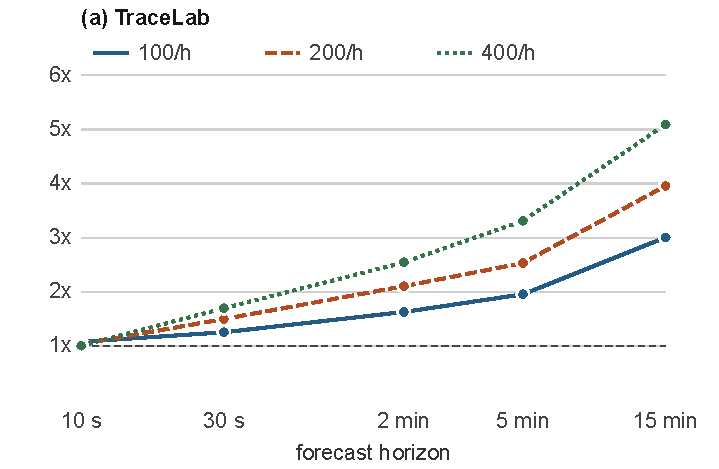
\includegraphics[width=.49\linewidth]{h1-tracelab.pdf}\hfill
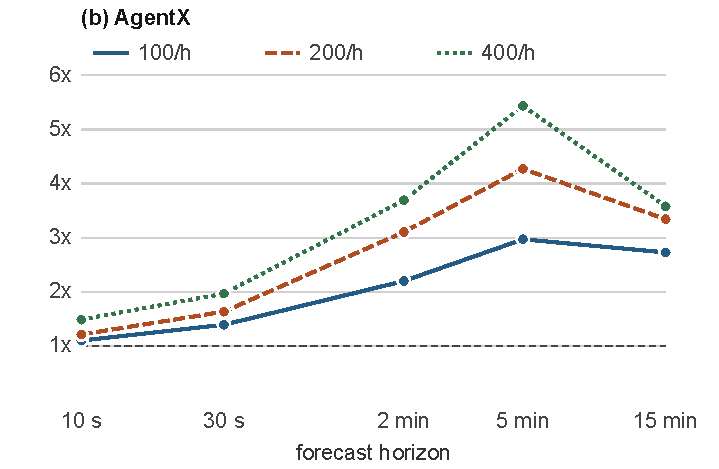
\includegraphics[width=.49\linewidth]{h1-agentx.pdf}
\caption{H1a sweep: ratio of mean B1 loss to mean M1 loss across seeds 0-2, at three overlay arrival rates. Ratios above one favor M1. The horizontal axis is logarithmic; line styles also distinguish rates. These are point estimates, with no confidence interval for the ratio. The near-unity TraceLab values at 10 seconds do not imply consistent improvement on individual seeds.}
\label{fig:2}
\end{figure}


Across the sweep, ratios at five minutes range from 1.96 to 3.31 on TraceLab and from 2.97 to 5.43 on AgentX (Figure~\ref{fig:2}). At fifteen minutes, the ranges are 3.00-5.09 and 2.73-3.58, respectively. AgentX's advantage therefore does not increase monotonically with horizon. Three seeds provide limited precision: the stored normal-approximation interval half-widths for M1's fifteen-minute AgentX loss are approximately 51-63\% of its mean. These intervals describe the component loss, not the plotted ratio.


The recorded TraceLab analysis attributes 81-99\% of demand to sessions already in flight over the tested horizons, consistent with the opportunity for session-aware forecasting. However, nominal 90\% intervals from the session model cover only approximately 40-73\% of observations. Training-only dispersion calibration increases coverage to approximately 65-86\% and worsens short-horizon pinball loss in the recorded calibration run. Residual bias, dependence, and distribution shift are plausible explanations; these results do not identify which mechanism dominates. B2 performs poorly in the heterogeneous fleet experiments, supporting survival conditioning for this predictor rather than establishing the inferiority of every TTL-based cache policy.


\subsection{H1b: progress helps, but depends on the tool's progress curve}
\label{sec:6.2}
\begin{figure}[!htbp]
\centering
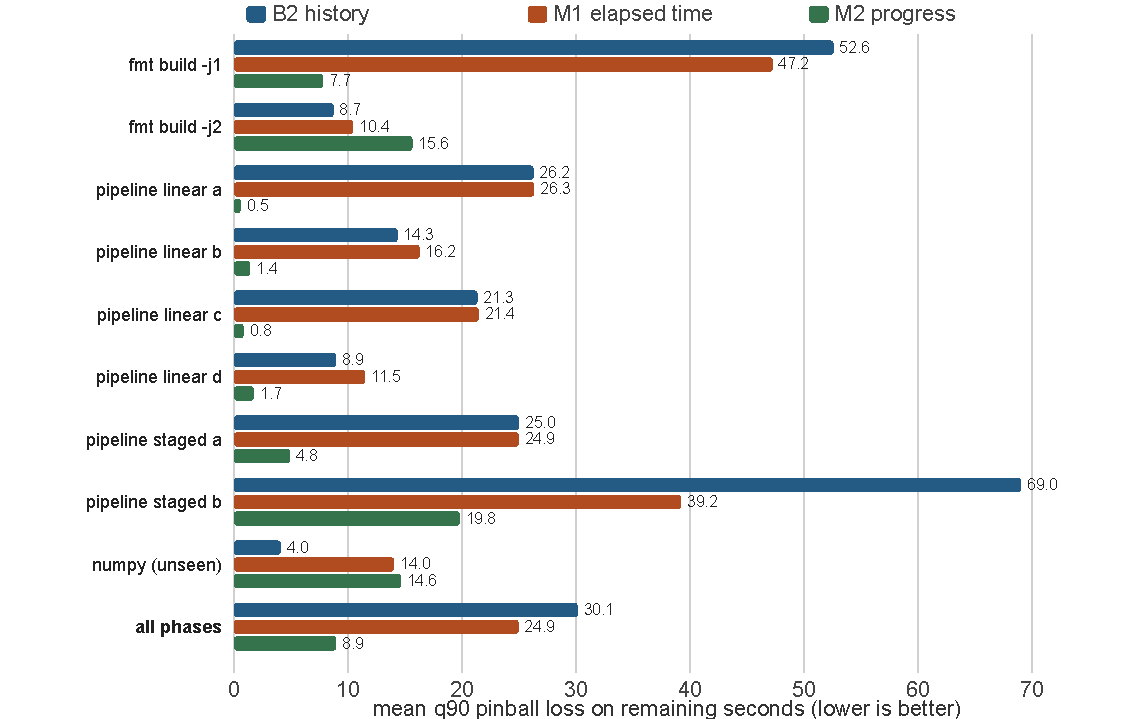
\includegraphics[width=.92\linewidth]{h1b-progress.pdf}
\caption{Leave-one-job-family-out remaining-time evaluation. Bars show mean q90 pinball loss in seconds; lower is better. The aggregate weights all 202 observation points equally. The NumPy family is unseen in training for its displayed row. Bars are descriptive averages, not estimates from independent observations with uncertainty bars.}
\label{fig:3}
\end{figure}


Across the retained collection, M2 reduces mean q90 pinball loss from M1's 24.9 to 8.9 seconds, a 2.80-fold loss ratio (64\% reduction). CRPS decreases from 59.0 to 30.1 seconds, a 1.96-fold ratio. The larger CRPS ratio of 3.4 recorded for an earlier pipeline/build-only collection does not apply to the expanded collection shown here.


Progress is most informative for the linear pipelines, whose M2 losses range from 0.5 to 1.7 seconds. It remains useful with four stage markers, but is not uniformly beneficial: M2 loses to M1 for the fmt \path{-j2} build and the held-out NumPy suite. Reported work fractions can map nonlinearly to elapsed time, and a curve learned from a different build configuration can be misleading. A separate one-prior-run NumPy analysis in the research notes reports CRPS of 18.8 seconds for M2 versus 53.7 for M1; that is a different training protocol and is not pooled into Figure~\ref{fig:3}.


The results support the value of progress on the measured jobs, not on arbitrary external actions. The sample contains nine scored families on one machine, with repeated observations within phases and limited environmental variation. The current implementation can key progress curves by command signature, but the retained score file predates evaluation of that change. Its results must not be attributed to the newer signature-aware implementation.


\subsection{H2: loaded short-interactive workloads show a latency-cost trade-off}
\label{sec:6.3}
In the loaded long-tool regime, interactive sessions still execute short shell tools. Forecast M2 raises session-weighted SLO attainment from 85.3\% to 94.6\% (Table~\ref{tab:5}). Its paired improvement is 9.3 percentage points, with a 95\% session-bootstrap interval of 8.0-10.5 points. Mean background JCT rises from 3,310 to 4,100 seconds, approximately 24\%. The corresponding bootstrap estimate of the difference is 789 seconds [739, 837].


\begin{table}[!htbp]
\centering
\caption{Loaded long-tool regime, three seeds. SLO is session-weighted attainment (\%); \(\Delta\)SLO is in percentage points. JCT is mean background completion time (s). Brackets are paired 95\% session-bootstrap intervals.}
\label{tab:5}
\small
\setlength{\tabcolsep}{4pt}
\begin{tabular*}{\linewidth}{@{\extracolsep{\fill}}lrrrr@{}}
\toprule
\thead[l]{Arm} & \thead{SLO (\%)} & \thead{\(\Delta\)SLO [95\% interval]} & \thead{JCT (s)} & \thead{\(\Delta\)JCT [95\% interval]} \\
\midrule
Native & 85.3 & - & 3,310 & - \\
Rules & 86.7 & +1.4 [-0.2, +2.8] & 3,278 & -35 [-90, +17] \\
Forecast M1 & 94.1 & +8.8 [+7.4, +10.1] & 4,101 & +790 [+736, +842] \\
Forecast M2 & 94.6 & +9.3 [+8.0, +10.5] & 4,100 & +789 [+739, +837] \\
M2, no holds & 84.1 & -1.3 [-2.8, +0.1] & 3,277 & -35 [-97, +10] \\
Heap lookahead & 92.3 & +7.0 [+5.4, +8.3] & 4,453 & +1141 [+1090, +1190] \\
Working set & 92.9 & +7.6 [+6.3, +8.9] & 5,392 & +2082 [+2035, +2136] \\
\bottomrule
\end{tabular*}
\end{table}


\begin{figure}[!htbp]
\centering
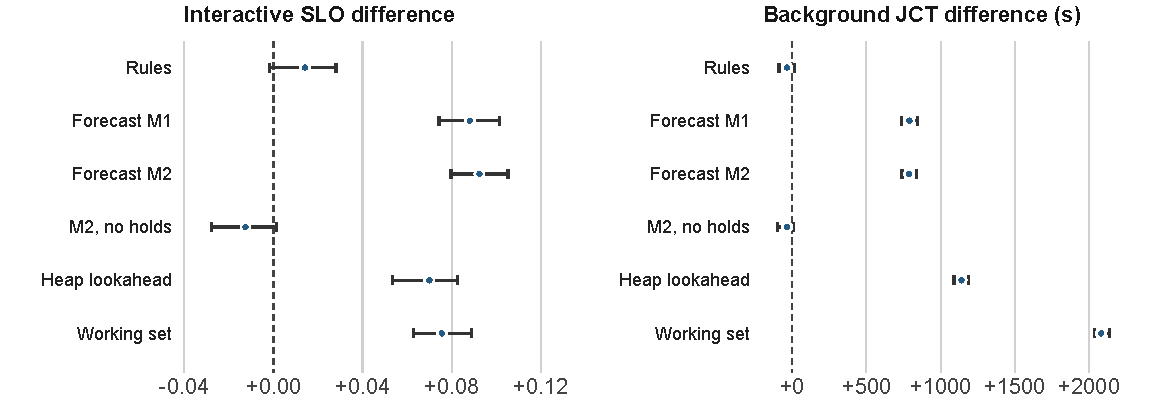
\includegraphics[width=1\linewidth]{h2-tradeoff.pdf}
\caption{Paired differences from native in the loaded regime. Left: session-weighted SLO difference on the 0-1 scale. Right: mean background JCT difference in seconds. Points are bootstrap mean differences; lines are 95\% session-bootstrap intervals. Positive SLO differences are beneficial; positive JCT differences are costs.}
\label{fig:4}
\end{figure}


Removing holds from M2 eliminates the observed SLO gain over native in this regime. This supports a role for the hold mechanism in the measured trade-off; it does not prove that the particular forecast is necessary or that another hold heuristic could not obtain a similar result. M1 and M2 produce similar point estimates because the hold rule targets interactive demand over 30 seconds, while the distinctive long progress-emitting tools are in the background class.


The working-set arm reaches 92.9\% SLO attainment and adds 2,082 seconds of background JCT. Its incremental background cost is approximately 2.64 times that of M2, but the SLO outcomes are not identical. This is a comparison between local policies under one simulator configuration, not a claim of superiority over ThunderAgent. Neither lookahead nor working-set results provide an optimal policy bound.


Costs extend beyond JCT. Forecast M2 reduces background deadline attainment from 19.0\% to 12.2\%, accumulates approximately 4.20 million held KV block-seconds per seed, and reaches the hold cap on approximately 1,193 occasions per seed (Appendix~\ref{app:B}). Its recomputed prefill volume is lower than native's in this loaded regime. In the underloaded long- and short-tool regimes, near-saturated SLO attainment limits discrimination: forecast M2 adds about 16 and 20 seconds to background JCT, respectively, for little change in the SLO metric. Lower request latency is not sufficient evidence of a favorable overall policy trade-off.


\subsection{Long interactive tools do not establish an M2 policy advantage}
\label{sec:6.4}
The completed long-interactive-tool experiment adds progress-emitting tests and builds to interactive sessions and uses a 60-second cap. It also changes arrival rates to 300 interactive and 480 background sessions per hour. It is therefore a separate regime, not a controlled hold-cap ablation. Table~\ref{tab:6} includes all eight arms, including the same-rule lookahead comparison.


\begin{table}[!htbp]
\centering
\caption{Long-interactive-tool regime, three seeds, 60-second hold cap. Units and interval construction match Table~\ref{tab:5}.}
\label{tab:6}
\small
\setlength{\tabcolsep}{4pt}
\begin{tabular*}{\linewidth}{@{\extracolsep{\fill}}lrrrr@{}}
\toprule
\thead[l]{Arm} & \thead{SLO (\%)} & \thead{\(\Delta\)SLO [95\% interval]} & \thead{JCT (s)} & \thead{\(\Delta\)JCT [95\% interval]} \\
\midrule
Native & 86.7 & - & 2,309 & - \\
Rules & 88.7 & +2.0 [+0.6, +3.8] & 2,359 & +48 [-5, +100] \\
Forecast M1 & 88.2 & +1.5 [+0.0, +3.0] & 2,585 & +275 [+228, +321] \\
Forecast M2 & 87.7 & +1.1 [-0.5, +2.5] & 2,604 & +293 [+244, +340] \\
M2, no holds & 86.8 & +0.1 [-1.4, +1.7] & 2,370 & +60 [+16, +115] \\
Heap lookahead & 87.4 & +0.8 [-0.7, +2.2] & 3,274 & +962 [+899, +1031] \\
Same-rule lookahead & 87.7 & +1.0 [-0.4, +2.6] & 3,315 & +1003 [+941, +1075] \\
Working set & 89.3 & +2.6 [+1.0, +3.9] & 2,921 & +611 [+557, +676] \\
\bottomrule
\end{tabular*}
\end{table}


M2's SLO improvement over native is 1.1 percentage points, with an interval spanning zero (-0.5 to 2.5 points), while its background JCT cost is 293 seconds [244, 340]. Rules-only admission has a higher SLO point estimate, 88.7\% versus 87.7\%, and a smaller JCT increase of 48 seconds [-5, 100]. M1 also has a higher SLO point estimate than M2. These native-referenced intervals do not directly test M1 against M2, but the results provide no evidence that progress-based forecasting improves this controller's performance.


The same-rule lookahead arm reaches 87.7\% SLO attainment with approximately 1,003 seconds of additional background JCT. More future information is thus not sufficient for this heuristic to improve the measured trade-off. Policy choice, horizon, and capacity approximation remain material limitations.


\subsection{A controlled cap ablation removes the loaded-regime gain}
\label{sec:6.5}
The 60-second-cap run repeats the loaded long-tool regime of Table~\ref{tab:5} with the same programs, seeds, engine and rates, changing only the hold cap from 600 to 60 seconds and adding the same-rule lookahead arm. It is the fixed-workload hold-cap ablation that Section~\ref{sec:6.4} could not provide.


\begin{table}[!htbp]
\centering
\caption{Loaded long-tool regime at a 60-second hold cap, three seeds. Units and interval construction match Table~\ref{tab:5}; the native row is the same workload as Table~\ref{tab:5} and differs only by bootstrap resampling.}
\label{tab:7}
\small
\setlength{\tabcolsep}{4pt}
\begin{tabular*}{\linewidth}{@{\extracolsep{\fill}}lrrrr@{}}
\toprule
\thead[l]{Arm} & \thead{SLO (\%)} & \thead{\(\Delta\)SLO [95\% interval]} & \thead{JCT (s)} & \thead{\(\Delta\)JCT [95\% interval]} \\
\midrule
Native & 85.3 & - & 3,310 & - \\
Rules & 86.7 & +1.4 [-0.2, +2.8] & 3,278 & -35 [-90, +17] \\
Forecast M1 & 85.2 & -0.1 [-1.6, +1.5] & 3,436 & +124 [+68, +180] \\
Forecast M2 & 84.3 & -1.0 [-2.4, +0.4] & 3,448 & +136 [+81, +187] \\
M2, no holds & 84.1 & -1.3 [-2.8, +0.1] & 3,277 & -35 [-97, +10] \\
Heap lookahead & 85.2 & -0.1 [-1.5, +1.3] & 4,461 & +1150 [+1085, +1213] \\
Same-rule lookahead & 84.2 & -1.1 [-2.4, +0.4] & 4,474 & +1162 [+1099, +1226] \\
Working set & 87.0 & +1.7 [+0.2, +3.2] & 3,815 & +505 [+445, +566] \\
\bottomrule
\end{tabular*}
\end{table}


With the cap at 60 seconds the forecast arms' SLO differences from native are -0.1 and -1.0 percentage points with intervals spanning zero, while their background JCT still rises by 124 seconds [68, 180] and 136 seconds [81, 187], and they accumulate approximately 3.7 million held KV block-seconds per seed with about 2,770 holds reaching the cap. The same-rule lookahead, holding with the true first-resumption demand in hand, changes SLO by -1.1 points [-2.4, +0.4] at a cost of 1,162 seconds [1,099, 1,226]. Rules-only admission is unchanged from Table~\ref{tab:5}. The working-set arm also responds to the shorter cap: its SLO attainment falls from 92.9\% to 87.0\%, while mean background JCT falls from 5,392 to 3,815 seconds. The 9.3-point gain of Table~\ref{tab:5} therefore depended on holds of up to ten minutes: what moved the interactive tail was sustained deferral of most background work, an effect available to any policy that defers that much, rather than the forecast's content.


A second reading follows from the hold counts. Under load the rule compares forecast demand with capacity that is free at the instant of decision, which is near zero at every instant, so its decision is almost always to hold regardless of the forecast; M1 and M2 cannot separate through a decision that does not depend on them. A revised rule that counts capacity expected to free within the slot has been implemented and is being rerun on both loaded regimes; those results are not part of this revision. Together, the three loaded runs support a conditional answer to H2: forecast-based holds as implemented do not improve serving under either load pattern at the proxy's intended 60-second cap, and the case for acting on the forecast, if there is one, lies in KV placement rather than admission.


\section{Discussion and Limitations}
\label{sec:7}
\textbf{Simulation validity.} No reported policy experiment runs on a real GPU. The engine model omits important effects of actual kernels, batching, memory movement, and interconnects. Fixed service rates and simplified cache eviction can affect even the relative ordering of policies. The simulator's metadata exposes the programmed output length to service-time estimation, which further simplifies deployment uncertainty. Mocker integration establishes request-path compatibility only.


\textbf{Target-to-control mismatch.} First-resumption KV demand is not simultaneous memory occupancy, and input-token demand is not uncached prefill work. Comparing these quantities with available capacity is a useful heuristic to study, but forecast calibration alone cannot validate that comparison. Repeated turns, cache sharing, backend interference, and multi-level fan-out require richer models. The present forecaster models only one level of fan-out.


\textbf{External validity and uncertainty.} Poisson-overlaid traces preserve within-session timing while changing fleet-level arrivals. Both public corpora represent coding agents, and AgentX gaps mix tool and human delays. Tool collections favor observable, parseable progress and do not cover silent tools, network services, or human actions broadly. Three seeds, dependent sessions in shared queues, and repeated H1b observations limit uncertainty estimates. The confidence intervals should not be interpreted as population-level guarantees.


\textbf{Baseline scope and attribution.} The study compares selected local baselines with particular parameter settings, without broad controller tuning or a matched reactive-hold baseline. B2 is an information ablation, not Continuum. The working-set arm is inspired by program pausing, not a faithful ThunderAgent implementation. The no-hold ablation measures the effect of holds within M2; it cannot isolate the value of the forecast from all alternative hold strategies. The event-heap lookahead arms neither optimize a common objective nor reveal all counterfactual future arrivals.


\textbf{Required validation.} A hardware study should compare native priority, rules, forecast policies, matched reactive holds, and published implementations on a common workload, reporting latency, completion time, task quality, and cache costs. The repository proposes a two-H100 Dynamo setup with instrumented background tools and interactive agents. Before such a study, paired simulation/hardware calibration, more seeds, signature-aware progress evaluation, and a hold rule whose decision depends on the forecast under load (Section~\ref{sec:6.5}) would clarify which findings transfer; the fixed-workload cap ablation has been run and is reported in Section~\ref{sec:6.5}. Explicit KV placement and predictive replica control remain future work.


\section{Conclusion}
\label{sec:8}
ATFM treats external agent execution as observable state for inference-demand forecasting. Across two coding-agent corpora, elapsed-time conditioning improves medium-horizon first-resumption forecasts over an aggregate-history baseline. Live progress further improves remaining-time scores on selected long-running tools, with identifiable failures when progress curves differ between training and evaluation. Closed-loop results are negative for the admission lever as implemented: forecast-based holds improve interactive SLO attainment only when the cap permits ten-minute deferrals, a controlled cap ablation removes the gain, and true future demand does not restore it, while rules-only admission gives a small consistent gain at little cost. The principal finding is that session state is useful for forecasting, while converting that information into a favorable serving policy remains workload- and controller-dependent.


\FloatBarrier
\bibliographystyle{unsrtnat}
\bibliography{references}

\clearpage
\appendix
\section{Artifact and Reproducibility}
\label{app:A}
\setcounter{table}{0}
\renewcommand{\thetable}{A\arabic{table}}
The editable manuscript is \path{docs/paper/atfm-paper.tex}, with BibTeX references in \path{references.bib} and vector PDF figures in \path{latex-fig/}. Tables and figures retain the values in the frozen CSVs under \path{docs/paper/results/}. The LaTeX document builds directly with \texttt{latexmk}; the optional \path{build_latex.py} wrapper checks compilation and publishes the PDF. Its \texttt{--figures} option refreshes vector figures from the saved result summaries. That directory includes a manifest with original run paths, source hashes, and the repository commit at capture. Raw \path{data/} and \path{runs/} directories are ignored by Git, so retaining these summaries makes paper rebuilding independent of locally collected raw traces. It does not by itself reproduce the experiments.


The repository specifies Python 3.12 and locks dependencies with \path{uv.lock}. The principal implementation paths are \path{src/atfm/board/} for session models and aggregation, \path{sidecar/} for tool observation, \path{proxy/} for admission, \path{sim/} for closed-loop execution, and \path{eval/} for scores and bootstrap metrics. Experiment configurations reside in \path{experiments/}. The architecture specification and dated research notes in \path{docs/} provide design history; when a narrative note disagrees with retained metrics, this report uses the metric files.


\begin{table}[!htbp]
\centering
\caption{Provenance of the main results. Paths are relative to the repository root; the corresponding summaries are frozen with this paper.}
\label{tab:A1}
\small
\setlength{\tabcolsep}{4pt}
\begin{tabularx}{\linewidth}{@{}p{.22\linewidth}X@{}}
\toprule
\thead[l]{Result} & \thead{Source artifact} \\
\midrule
H1a original run & \path{runs/h1_tracelab_r200/metrics.csv} \\
H1a sweeps & \path{runs/sweep_tracelab.csv}; \path{runs/sweep_agentx.csv} \\
H1b retained collection & \path{runs/h1b_with_numpy.csv}, aggregated by family/model and by model \\
Loaded H2 & \path{runs/h2sim_long_tool_loaded/{metrics,paired}.csv} \\
Long-interactive H2 & \path{runs/h2sim_interactive_long/{metrics,paired}.csv} \\
Loaded H2, 60-second cap & \path{runs/h2sim_long_tool_loaded_cap60/{metrics,paired}.csv} \\
\bottomrule
\end{tabularx}
\end{table}


From the repository root, the following commands rebuild the document and show the experiment entry points. Experiment commands require their configured raw inputs and may be expensive; they are distinct from the paper build.


\begin{Verbatim}[fontsize=\footnotesize,breaklines=true]
python3 docs/paper/build_latex.py
uv run python scripts/run_h1.py experiments/h1_tracelab.yaml
uv run python scripts/sweep_h1.py experiments/h1_agentx.yaml \
  --seeds 0 1 2 --rates 100 200 400 --out runs/sweep_agentx.csv
uv run python scripts/h1b_resumption.py <collection-events.jsonl> \
  --min-duration 30 --offset 15 --out <scores.csv>
uv run python scripts/run_h2sim.py experiments/h2sim_loaded.yaml
uv run python scripts/run_h2sim.py experiments/h2sim_interactive_long.yaml
uv run python scripts/run_h2sim.py experiments/h2sim_loaded_cap60.yaml
\end{Verbatim}


The reported H1b aggregate combines the earlier build/pipeline collections with NumPy runs; recreating it requires the same collection composition and historical predictor implementation. The current command-signature feature can change rescored values. Earlier exploratory results and integration checks are documented in \path{docs/research/2026-09-22-h1-first-results.md}, \path{2026-09-23-h1-second-corpus-and-h1b.md}, \path{2026-09-23-l1-results.md}, and \path{2026-09-24-h2sim-first-results.md}. The completed loaded 60-second-cap experiment is reported in Section~\ref{sec:6.5}; subsequent revised-controller experiments are outside this evidence snapshot.


\textbf{Writing assistance.} Earlier project materials disclosed assistance from Claude Code. This revision used Codex for editorial revision, consistency checks, and document generation; retained experiment summaries are identified above.


\section{Additional Loaded-Regime Costs}
\label{app:B}
\setcounter{table}{0}
\renewcommand{\thetable}{B\arabic{table}}
\begin{table}[!htbp]
\centering
\caption{Loaded long-tool regime. TTFT is the arithmetic mean of per-seed p95 values, not the p95 of pooled calls. Deadline attainment is pooled over common sessions. Recomputed prefill and held-cache occupancy are in millions per seed; cap counts are means per seed.}
\label{tab:B1}
\small
\setlength{\tabcolsep}{4pt}
\begin{tabular*}{\linewidth}{@{\extracolsep{\fill}}lrrrrr@{}}
\toprule
\thead[l]{Arm} & \thead{p95 TTFT\\(s)} & \thead{Deadline\\(\%)} & \thead{Recompute\\(M tokens)} & \thead{Held KV\\(M block-s)} & \thead{At cap} \\
\midrule
Native & 2.67 & 19.0 & 47.94 & 0.00 & 0 \\
Rules & 3.01 & 24.7 & 38.17 & 0.00 & 0 \\
Forecast M1 & 2.16 & 11.9 & 43.28 & 4.22 & 1,218 \\
Forecast M2 & 2.12 & 12.2 & 43.14 & 4.20 & 1,193 \\
M2, no holds & 3.23 & 24.3 & 41.38 & 0.00 & 0 \\
Heap lookahead & 2.51 & 9.1 & 41.03 & 2.18 & 805 \\
Working set & 2.29 & 11.4 & 46.58 & 0.00 & 1,096 \\
\bottomrule
\end{tabular*}
\end{table}


These metrics measure different aspects of the policy cost. Recomputed prefill counts work after eviction; held KV block-seconds integrate resident memory during a policy hold. A zero value in the working-set arm's held-KV column does not imply zero delay or zero cache cost: that policy can evict paused state. Cap counts denote imposed holds reaching the configured limit and do not bound subsequent window queueing.


\end{document}
